\subsection{Figures}
The following code excerpt is to insert a single figure into \LaTeX{} which will result in Figure~\ref{fig:h-vs-t}.

\begin{lstlisting}
\begin{figure}[!htbp]
\centering
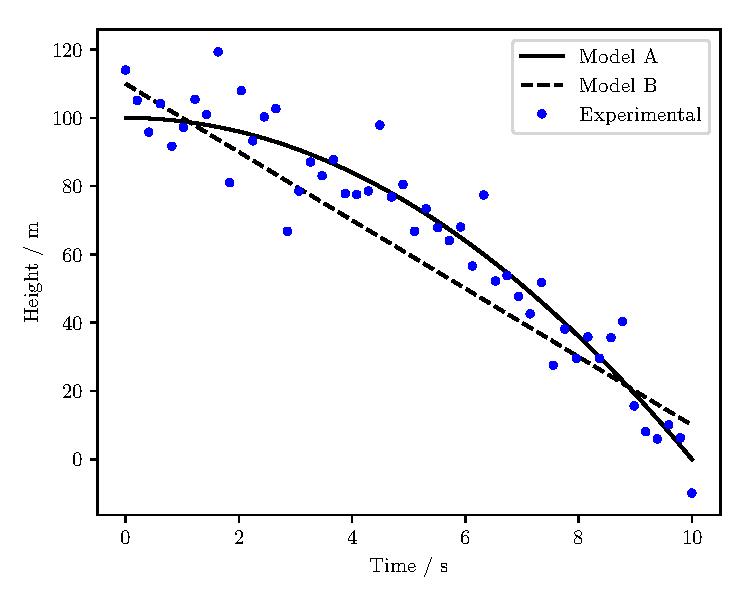
\includegraphics[width= 0.6\textwidth]{Figures/Height.pdf}
\caption[I don't have a list of figures]{Properly formatted graph.}
\label{fig:h-vs-t}
\end{figure}
\end{lstlisting}

\begin{figure}[!htbp]
\centering
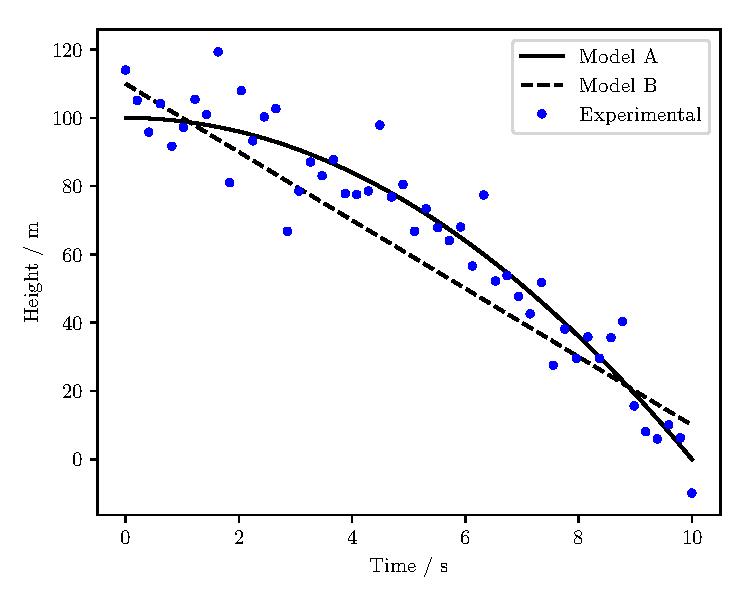
\includegraphics[width= 0.6\textwidth]{Figures/Height.pdf}
\caption[I don't have a list of figures]{Properly formatted graph.}
\label{fig:h-vs-t}
\end{figure}

The htbp refers to the placement of the figure in the order: here, top, bottom or next page. \LaTeX\ will do what it finds best, but adding an ! will force it to do what you say and not what it feels is best.

The centering command centre-aligns the figure. The third line is where the figure is actually inserted by using its filename as stated in the Figures subfolder. The square brackets are for command options; in this case the figure width is set to 60 \% of the text width. 

Likewise the caption has two parts. The caption in square brackets is what will be displayed in the list of figures (if needed) and the caption in curly brackets will be displayed below the figure. If these two are the same, you may simply leave out the square brackets. The label is the variable name for the figure and is used to reference the figure in-text \textit{eg}: $\backslash$ref\{fig:h-vs-t\}. The label name can be made anything, but \textsf{fig}, \textsf{fig} and \textsf{eq} are simply used to group the labels for similar objects together to find it easier in the suggestion box. In-text referencing is done by simply using the \texttt{ref} command. Precede it with a tilde for a nonbreaking space.



To insert two figures alongside each other, use a minipage environment. Two minipages are created in a figure environment with the width of each mini page less than 50 \% of the text width or else the figures will be below each other.

\begin{figure}[!htbp]
\centering
\begin{minipage}[t]{0.48\textwidth} 
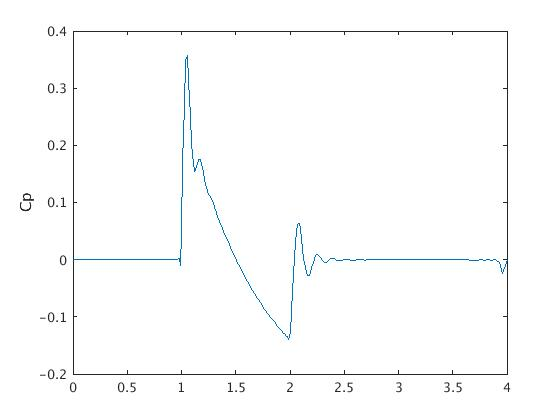
\includegraphics[width= \textwidth]{Figures/cp.jpg}
\caption{Pressure coefficient against airfoil.}
\label{fig:cp}
\end{minipage}
\begin{minipage}[t]{0.48\textwidth} 
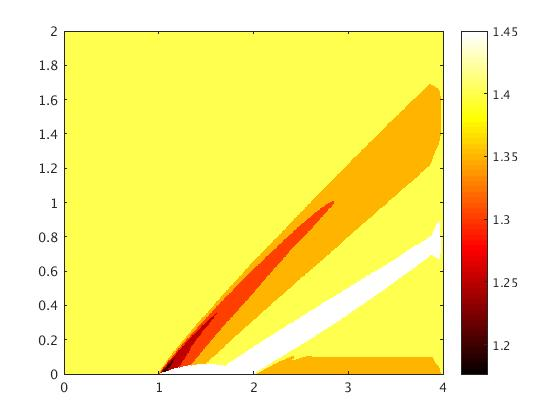
\includegraphics[width= \textwidth]{Figures/machcontour.jpg}
\caption{Mach number against the airfoil.}
\label{fig:mach}
\end{minipage}
\end{figure}    

\newpage
\subsection{Mathematics}
The excerpt below is to insert an equation:
\begin{lstlisting}
\begin{equation}
\dfrac{\partial \rho}{\partial t} + \nabla \cdot (\rho \bar{u}) = 0
\label{eq:continuity}
\end{equation}
\end{lstlisting}

For equations, Greek symbols can be entered by typing the name of the symbol (use a capital letter if an upper case letter is required). Refer to \href{https://www.sharelatex.com/learn/List_of_Greek_letters_and_math_symbols}{www.sharelatex.com} for more information on Greek and mathematical symbols. Consider Equation~\ref{eq:continuity}, Equation~\ref{eq:ftc}, and Equation~\ref{eq:taylor}

\begin{equation}
\label{eq:continuity}
\frac{\partial \rho}{\partial t} + \nabla \cdot (\rho \bar{u}) = 0
\end{equation}
\nomenclature{$\rho$}{Density (\si{\kilo \gram \per \cubic \meter})}
\nomenclature{$t$}{Time (\si{\second})}
\nomenclature{$u$}{Velocity (\si{\meter \per \second})}

\begin{equation}
\label{eq:ftc}
f(x) = \frac{\mathrm{d}}{\mathrm{d}x} \int^\infty_0  f(s) \, \mathrm{d}s
\end{equation}

\begin{equation}
\label{eq:taylor}
\sum^\infty_{n=0} \frac{f^{(n)}(a)}{n!} (x-a)^n
\end{equation}

Here are examples of chemical reactions

\begin{eqnarray*}
  \ce{A + 2B &<=>& AB2} \\
  \ce{MgCl_2 {\cdot} 6 H_2O &\xrightarrow{69 \; {\degree C}}& MgCl_2 {\cdot} 4 H_2O + 2H_2O} \\
\end{eqnarray*}

\subsection{Tables}
The main structure of the table is similar to that of a figure. Once again the code is enclosed by a begin and end command, a caption, and a label at the top. The excerpt below creates Table~\ref{tab:fpiorder}. The begin tabular command with three ls (lll) creates a table with left-aligned columns. The thicker top and bottom rules are made using the $\backslash$toprule and $\backslash$bottomrule commands. The thinner heading rule is made by using $\backslash$midrule. If you have a table of data from another program like Microsoft Excel, copy and paste them in the \href{https://www.tablesgenerator.com/}{\LaTeX{} Table Generator}.

\begin{lstlisting}
\begin{table}[!ht]
\centering
\caption{FPI rate and order of convergence}
\label{tab:fpiorder}
    \begin{tabular}{lll}
        \toprule
        k$_s$ & q & $\mu$ (cP) \\
        \midrule
        1 & 0.9940& -0.1761\\
        2 & 0.9887 & -0.2896\\
        4 & 0.9895& -0.4366\\
        \bottomrule
    \end{tabular}
\end{table}
\end{lstlisting}

\begin{table}[!ht]
    \centering
    \caption{FPI rate and order of convergence}
    \label{tab:fpiorder}
    \begin{tabular}{lll}
        \hlineB{3}
        k$_s$ (m s$^{-1}$) & q (W) & $\mu$ (cP) \\
        \midrule
        1 & 0.9940& -0.1761\\
        2 & 0.9887 & -0.2896\\
        4 & 0.9895& -0.4366\\
        \hlineB{3}  
    \end{tabular}
\end{table}

For a more advanced table, consider Table~\ref{tab:tabexample}.

\begin{table}[htbp]
\centering
\caption{Example of a table}
\label{tab:tabexample}
\begin{minipage}{0.5\textwidth}
\begin{centering}
\begin{tabular}{@{}llr@{}}
\toprule 
\multicolumn{2}{c}{Item} &            \\ \cline{1-2}
Animal     & Description & Price\textsuperscript{a} (\$) \\ 
\hline
Gnat       & per gram    & 13.65      \\
           & each        & 0.01       \\
Gnu        & stuffed     & 92.50      \\
Emu        & stuffed     & 33.33      \\
Armadillo  & frozen      & 8.99       \\ \bottomrule 
\end{tabular}

\vspace{1em}
\textsuperscript{a} As of 2004  
\end{centering} 
\end{minipage}
\end{table}


\subsection{Referencing}

When referencing literature, add your reference to the .bib file. To cite them in-text, use the commands in Table \ref{tab:Cite}.

\begin{table}[!ht]
\centering
\caption{In-text literature referencing examples}
\label{tab:Cite}
    \begin{tabular}{ll}
        \toprule
        \LaTeX\ syntax & Result\\
        \midrule
        $\backslash$parencite\{Bezuidenhoudt2017\} &\parencite{Bezuidenhoudt2017} \\
        $\backslash$textcite\{Bezuidenhoudt2017\} & \textcite{Bezuidenhoudt2017} \\
        $\backslash$parencite[250]\{Cengel2015\} &\parencite[250]{Cengel2015} \\
        $\backslash$textcite[250]\{Cengel2015\} & \textcite[250]{Cengel2015} \\
        \bottomrule
    \end{tabular}
\end{table}

This will create your reference list correct according to the departmental guidelines. Below is an example of a book and an article reference. For more examples see the \href{https://www.verbosus.com/bibtex-style-examples.html}{BibTeX Style Examples} website. 

\begin{lstlisting}
@Book{cengel2015,
  author		= {\c{C}engel, Y A and Ghajar, A J},
  title			= {Heat and Mass Transfer},
  publisher		= {McGraw-Hill},
  year			= 2015,
  address		= {New York},
  edition		= 5
}

@Article{Bezuidenhoudt2017,
  author   = {Bezuidenhoudt, A and Sonnendecker, PW and Crouse, PL},
  title	   = {Temperature and pressure effects on the product distribution of PTFE pyrolysis by means of qualitative, in-line FTIR analysis},
  journal  = {Polymer Degradation and Stability},
  year	   = 2017,
  pages	   = {79-88},
  volume   = {142}
}
\end{lstlisting}

To create a reference list at the end of your document, simply type: 
\begin{lstlisting}
\printbibliography
\end{lstlisting} 
\nocite{*}